\documentclass{standalone}
\usepackage{tikz}
\usetikzlibrary{patterns, positioning}

\begin{document}
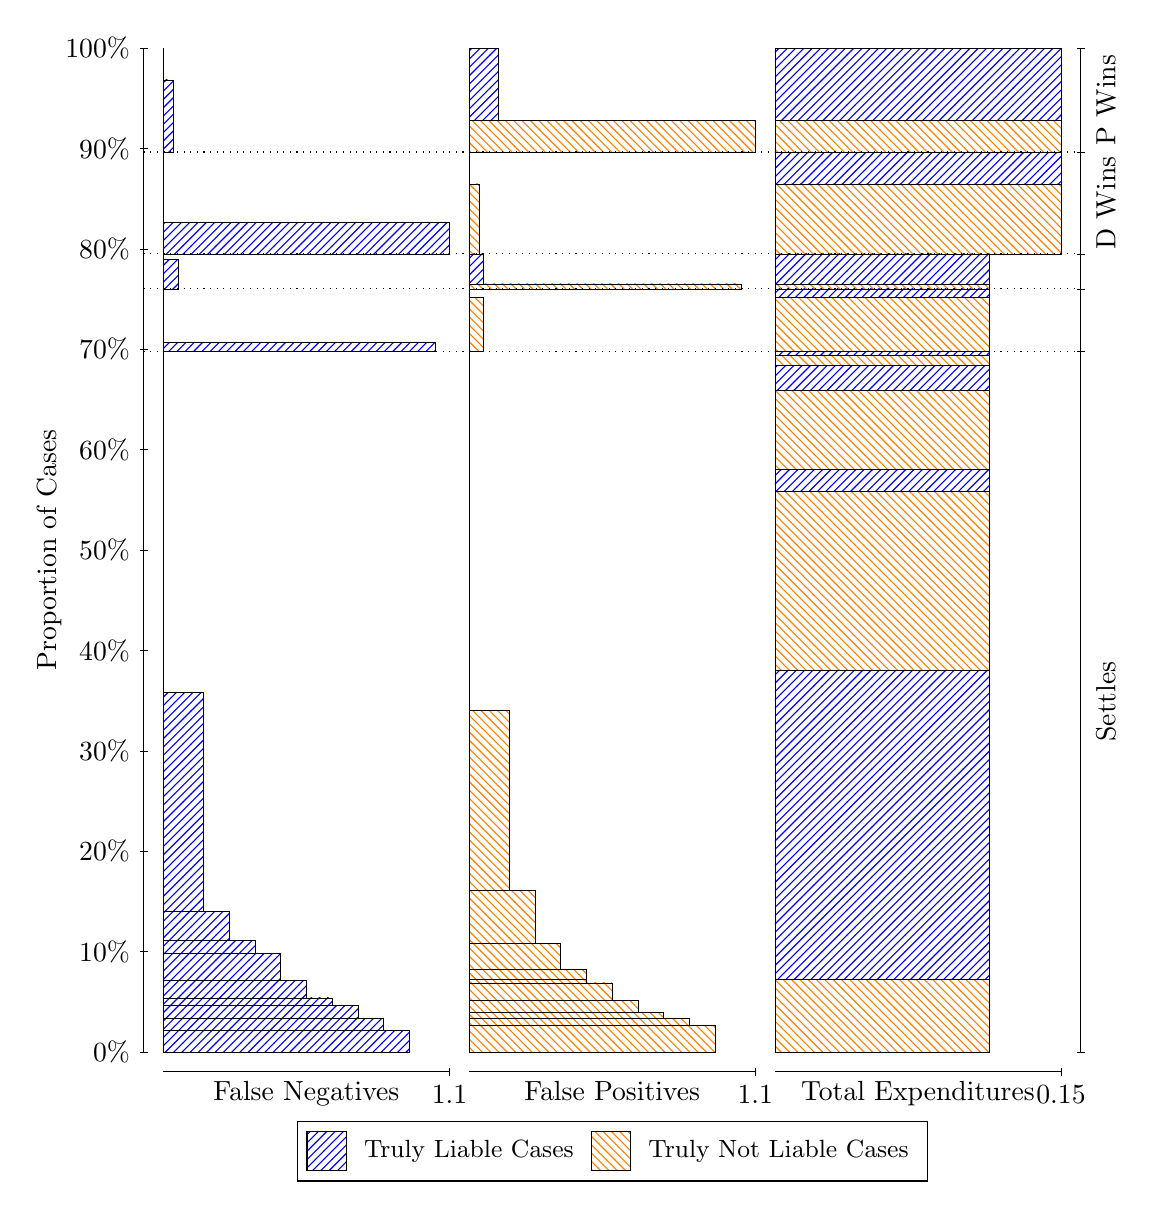
\begin{tikzpicture}
\draw[black, very thin] (1.5,1.75) -- (1.5,14.5);
\node[rotate=90, anchor=center] at (0.3, 8.125) {Proportion of Cases};
\draw[black, very thin] (1.45,1.75) -- (1.55,1.75);
\node[anchor=east] at (1.45, 1.75) {0\%};
\draw[black, very thin] (1.45,3.025) -- (1.55,3.025);
\node[anchor=east] at (1.45, 3.025) {10\%};
\draw[black, very thin] (1.45,4.3) -- (1.55,4.3);
\node[anchor=east] at (1.45, 4.3) {20\%};
\draw[black, very thin] (1.45,5.575) -- (1.55,5.575);
\node[anchor=east] at (1.45, 5.575) {30\%};
\draw[black, very thin] (1.45,6.85) -- (1.55,6.85);
\node[anchor=east] at (1.45, 6.85) {40\%};
\draw[black, very thin] (1.45,8.125) -- (1.55,8.125);
\node[anchor=east] at (1.45, 8.125) {50\%};
\draw[black, very thin] (1.45,9.4) -- (1.55,9.4);
\node[anchor=east] at (1.45, 9.4) {60\%};
\draw[black, very thin] (1.45,10.675) -- (1.55,10.675);
\node[anchor=east] at (1.45, 10.675) {70\%};
\draw[black, very thin] (1.45,11.95) -- (1.55,11.95);
\node[anchor=east] at (1.45, 11.95) {80\%};
\draw[black, very thin] (1.45,13.225) -- (1.55,13.225);
\node[anchor=east] at (1.45, 13.225) {90\%};
\draw[black, very thin] (1.45,14.5) -- (1.55,14.5);
\node[anchor=east] at (1.45, 14.5) {100\%};

\draw[black, very thin] (13.4,1.75) -- (13.4,14.5);
\draw[black, very thin] (13.35,1.75) -- (13.45,1.75);
\node[anchor=west] at (13.35, 1.75) {};
\draw[black, very thin] (13.35,10.651) -- (13.45,10.651);
\node[anchor=west] at (13.35, 10.651) {};
\draw[black, very thin] (13.35,11.441) -- (13.45,11.441);
\node[anchor=west] at (13.35, 11.441) {};
\draw[black, very thin] (13.35,11.885) -- (13.45,11.885);
\node[anchor=west] at (13.35, 11.885) {};
\draw[black, very thin] (13.35,13.179) -- (13.45,13.179);
\node[anchor=west] at (13.35, 13.179) {};
\draw[black, very thin] (13.35,14.5) -- (13.45,14.5);
\node[anchor=west] at (13.35, 14.5) {};

\draw[black, very thin, pattern color=blue, pattern=north east lines] (1.75,1.75) rectangle (4.873,2.0222);
\draw[black, very thin, pattern color=blue, pattern=north east lines] (1.75,2.0222) rectangle (4.5464,2.1737);
\draw[black, very thin, pattern color=blue, pattern=north east lines] (1.75,2.1737) rectangle (4.2199,2.346);
\draw[black, very thin, pattern color=blue, pattern=north east lines] (1.75,2.346) rectangle (3.8933,2.4369);
\draw[black, very thin, pattern color=blue, pattern=north east lines] (1.75,2.4369) rectangle (3.5667,2.6626);
\draw[black, very thin, pattern color=blue, pattern=north east lines] (1.75,2.6626) rectangle (3.2401,3.0004);
\draw[black, very thin, pattern color=blue, pattern=north east lines] (1.75,3.0004) rectangle (2.9135,3.1644);
\draw[black, very thin, pattern color=blue, pattern=north east lines] (1.75,3.1644) rectangle (2.5869,3.5388);
\draw[black, very thin, pattern color=blue, pattern=north east lines] (1.75,3.5388) rectangle (2.2603,6.3173);
\draw[black, very thin, pattern color=orange, pattern=north west lines] (1.75,6.3173) rectangle (1.75,10.651);
\draw[black, very thin, pattern color=blue, pattern=north east lines] (1.75,10.651) rectangle (5.1996,10.758);
\draw[black, very thin, pattern color=orange, pattern=north west lines] (1.75,10.758) rectangle (1.75,11.441);
\draw[black, very thin, pattern color=blue, pattern=north east lines] (1.75,11.441) rectangle (1.9337,11.82);
\draw[black, very thin, pattern color=orange, pattern=north west lines] (1.75,11.82) rectangle (1.75,11.885);
\draw[black, very thin, pattern color=blue, pattern=north east lines] (1.75,11.885) rectangle (5.3833,12.29);
\draw[black, very thin, pattern color=orange, pattern=north west lines] (1.75,12.29) rectangle (1.75,13.179);
\draw[black, very thin, pattern color=blue, pattern=north east lines] (1.75,13.179) rectangle (1.8725,14.095);
\draw[black, very thin, pattern color=orange, pattern=north west lines] (1.75,14.095) rectangle (1.75,14.5);
\draw[black, very thin, pattern color=orange, pattern=north west lines] (5.6333,1.75) rectangle (8.7564,2.0919);
\draw[black, very thin, pattern color=orange, pattern=north west lines] (5.6333,2.0919) rectangle (8.4298,2.1796);
\draw[black, very thin, pattern color=orange, pattern=north west lines] (5.6333,2.1796) rectangle (8.1032,2.2554);
\draw[black, very thin, pattern color=orange, pattern=north west lines] (5.6333,2.2554) rectangle (7.7766,2.4004);
\draw[black, very thin, pattern color=orange, pattern=north west lines] (5.6333,2.4004) rectangle (7.45,2.6278);
\draw[black, very thin, pattern color=orange, pattern=north west lines] (5.6333,2.6278) rectangle (7.1234,2.6722);
\draw[black, very thin, pattern color=orange, pattern=north west lines] (5.6333,2.6722) rectangle (7.1234,2.8001);
\draw[black, very thin, pattern color=orange, pattern=north west lines] (5.6333,2.8001) rectangle (6.7968,3.133);
\draw[black, very thin, pattern color=orange, pattern=north west lines] (5.6333,3.133) rectangle (6.4702,3.8043);
\draw[black, very thin, pattern color=orange, pattern=north west lines] (5.6333,3.8043) rectangle (6.1436,6.0839);
\draw[black, very thin, pattern color=blue, pattern=north east lines] (5.6333,6.0839) rectangle (5.6333,10.651);
\draw[black, very thin, pattern color=orange, pattern=north west lines] (5.6333,10.651) rectangle (5.817,11.334);
\draw[black, very thin, pattern color=blue, pattern=north east lines] (5.6333,11.334) rectangle (5.6333,11.441);
\draw[black, very thin, pattern color=orange, pattern=north west lines] (5.6333,11.441) rectangle (9.083,11.506);
\draw[black, very thin, pattern color=blue, pattern=north east lines] (5.6333,11.506) rectangle (5.817,11.885);
\draw[black, very thin, pattern color=orange, pattern=north west lines] (5.6333,11.885) rectangle (5.7558,12.774);
\draw[black, very thin, pattern color=blue, pattern=north east lines] (5.6333,12.774) rectangle (5.6333,13.179);
\draw[black, very thin, pattern color=orange, pattern=north west lines] (5.6333,13.179) rectangle (9.2667,13.583);
\draw[black, very thin, pattern color=blue, pattern=north east lines] (5.6333,13.583) rectangle (6.0007,14.5);
\draw[black, very thin, pattern color=orange, pattern=north west lines] (9.5167,1.75) rectangle (12.242,2.6722);
\draw[black, very thin, pattern color=blue, pattern=north east lines] (9.5167,2.6722) rectangle (12.242,6.5934);
\draw[black, very thin, pattern color=orange, pattern=north west lines] (9.5167,6.5934) rectangle (12.242,8.873);
\draw[black, very thin, pattern color=blue, pattern=north east lines] (9.5167,8.873) rectangle (12.242,9.1453);
\draw[black, very thin, pattern color=orange, pattern=north west lines] (9.5167,9.1453) rectangle (12.242,10.15);
\draw[black, very thin, pattern color=blue, pattern=north east lines] (9.5167,10.15) rectangle (12.242,10.473);
\draw[black, very thin, pattern color=orange, pattern=north west lines] (9.5167,10.473) rectangle (12.242,10.601);
\draw[black, very thin, pattern color=blue, pattern=north east lines] (9.5167,10.601) rectangle (12.242,10.651);
\draw[black, very thin, pattern color=orange, pattern=north west lines] (9.5167,10.651) rectangle (12.242,11.334);
\draw[black, very thin, pattern color=blue, pattern=north east lines] (9.5167,11.334) rectangle (12.242,11.441);
\draw[black, very thin, pattern color=orange, pattern=north west lines] (9.5167,11.441) rectangle (12.242,11.506);
\draw[black, very thin, pattern color=blue, pattern=north east lines] (9.5167,11.506) rectangle (12.242,11.885);
\draw[black, very thin, pattern color=orange, pattern=north west lines] (9.5167,11.885) rectangle (13.15,12.774);
\draw[black, very thin, pattern color=blue, pattern=north east lines] (9.5167,12.774) rectangle (13.15,13.179);
\draw[black, very thin, pattern color=orange, pattern=north west lines] (9.5167,13.179) rectangle (13.15,13.583);
\draw[black, very thin, pattern color=blue, pattern=north east lines] (9.5167,13.583) rectangle (13.15,14.5);
\draw[black, dotted] (1.5,10.651) -- (13.4,10.651);
\draw[black, dotted] (1.5,11.441) -- (13.4,11.441);
\draw[black, dotted] (1.5,11.885) -- (13.4,11.885);
\draw[black, dotted] (1.5,13.179) -- (13.4,13.179);
\draw[black, very thin] (1.75,1.5) -- (5.3833,1.5);
\node[anchor=north] at (3.5667, 1.5) {False Negatives};
\draw[black, very thin] (5.3833,1.45) -- (5.3833,1.55);
\node[anchor=north] at (5.3833, 1.45) {1.1};

\draw[black, very thin] (5.6333,1.5) -- (9.2667,1.5);
\node[anchor=north] at (7.45, 1.5) {False Positives};
\draw[black, very thin] (9.2667,1.45) -- (9.2667,1.55);
\node[anchor=north] at (9.2667, 1.45) {1.1};

\draw[black, very thin] (9.5167,1.5) -- (13.15,1.5);
\node[anchor=north] at (11.333, 1.5) {Total Expenditures};
\draw[black, very thin] (13.15,1.45) -- (13.15,1.55);
\node[anchor=north] at (13.15, 1.45) {0.15};

\node[black, centered, rotate=90] at (13.72, 6.2006) {Settles};


\node[black, centered, rotate=90] at (13.72, 12.532) {D Wins};
\node[black, centered, rotate=90] at (13.72, 13.839) {P Wins};

\draw (7.449999999999999,1.5) node[draw=none] (baseCoordinate) {};
\begin{scope}[align=center]
        \matrix[scale=0.5, draw=black, below=0.5cm of baseCoordinate, nodes={draw}, column sep=0.1cm]{
            \node[rectangle, draw, minimum width=0.5cm, minimum height=0.5cm, pattern=north east lines, pattern color=blue] {}; &
            \node[draw=none, font=\small] (B) {Truly Liable Cases}; &
            \node[rectangle, draw, minimum width=0.5cm, minimum height=0.5cm, pattern=north west lines, pattern color=orange] {}; &
            \node[draw=none, font=\small] (B) {Truly Not Liable Cases}; \\
            };
\end{scope}

\end{tikzpicture}
\end{document}